\documentclass[a4paper,11pt,UTF8]{article}
\usepackage{ctex}
\usepackage{amsmath,amsthm,amssymb,amsfonts}
\usepackage{amsmath}
\usepackage[a4paper]{geometry}
\usepackage{graphicx}
\usepackage{microtype}
\usepackage{siunitx}
\usepackage{booktabs}
\usepackage[colorlinks=false, pdfborder={0 0 0}]{hyperref}
\usepackage{cleveref}
\usepackage{esint} 
\usepackage{graphicx}
\usepackage{ragged2e}
\usepackage{pifont}
\usepackage{extarrows}
\usepackage{mathptmx}
\usepackage{float}
\usepackage{caption}
\captionsetup[figure]{name={Figure}}

\title{Microelectronics Circuit Analysis and Design Homework(10th)}
\author{Yuejin Xie \quad U202210333}
\date{Oct 23rd, 2023}
\begin{document}
\maketitle
8.24 Consider the class-B output stage with complementary MOSFETs shown in Figure P8.24. The transistor parameters are $V_{TN}=V_{TP}=0$ and $K_n=K_p=$ $0.4$mA$/N^2$. Let $R_L=5$ k$\Omega$. (a) Find the maximum output voltage such that $M_n$ remains biased in the saturation region. What are the corresponding values of $i_L$ and $\upsilon_I$ for this condition? (b) Determine the conversion efficiency for a symmetrical sine-wave output signal with the peak value found in part (a).
\begin{figure}[H]
	\centering
	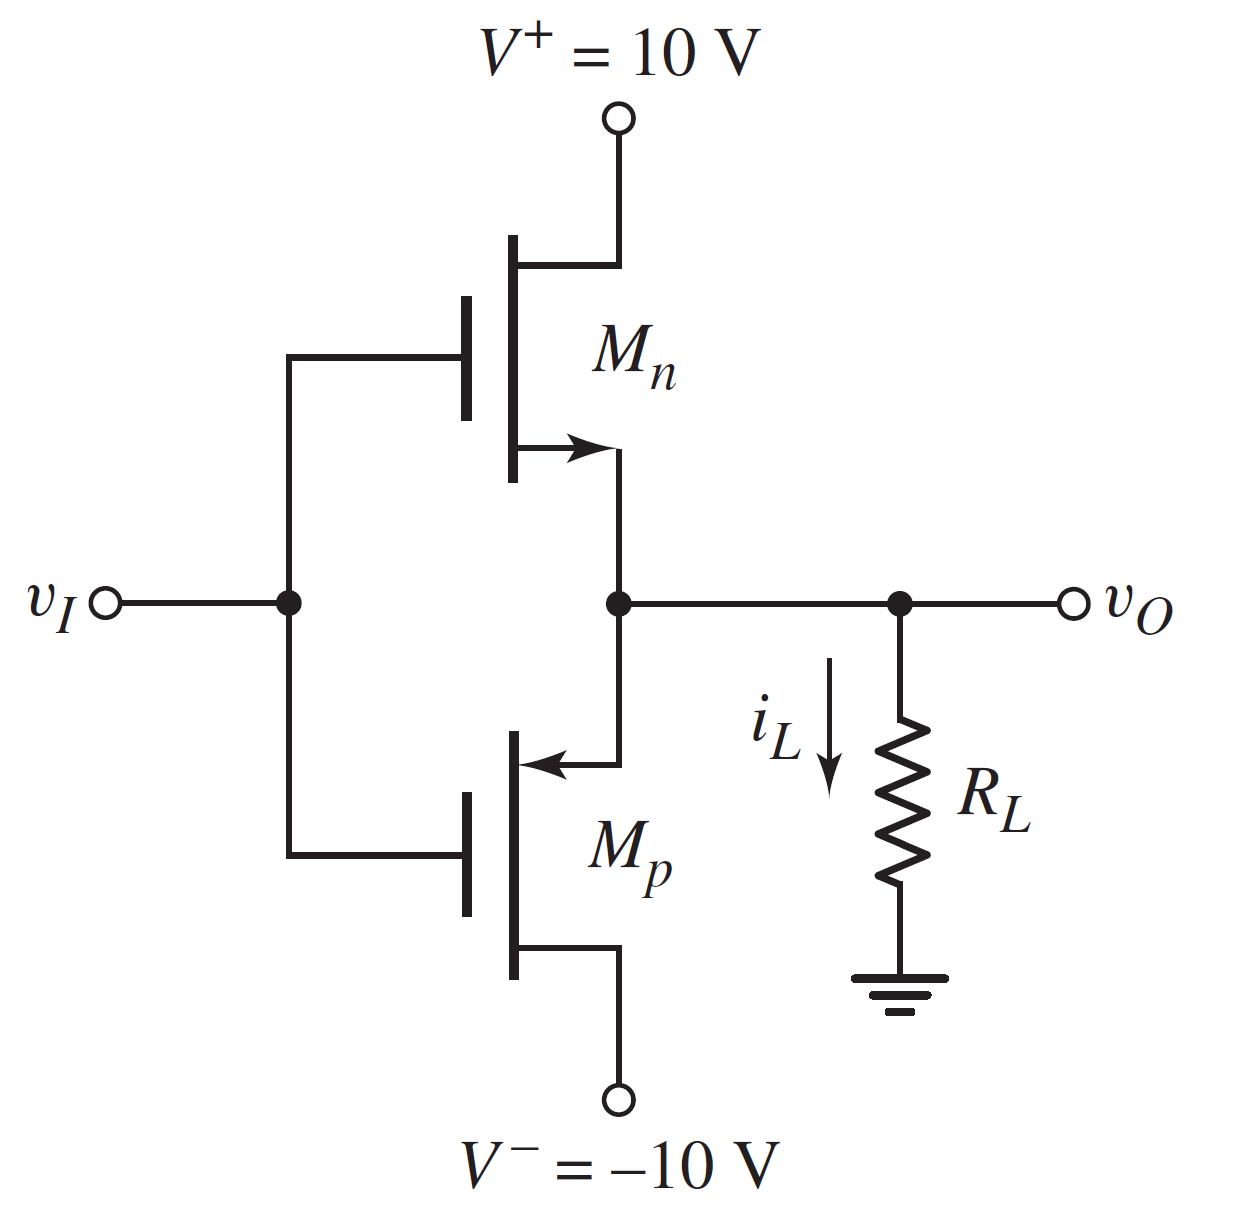
\includegraphics[width=0.5\textwidth]{8.24}
	\caption{Problem 8.24}
\end{figure}
8.29 An enhancement-mode MOSFET class-AB output stage is shown in Figure P8.29. The threshold voltage of each transistor is $V_{TN}=-V_{TP}=1$V and the conduction parameters of the output transistors are $K_{n1}=K_{p2}=$
5 mA/V$^{2}$. Let $I_{\text{Bias}}=200$ $\mu$ A. (a) Determine $K_{n3}=K_{p4}$ such that the quiescent drain currents in $M_1$ and $M_2$ are 5 mA. (b) Using the results of part (a), find the small-signal voltage gain $A_v=dv_O/dv_I$ evaluated at: (i) $v_O=0$, and (ii) $v_O=5$V.
\begin{figure}[H]
	\centering
	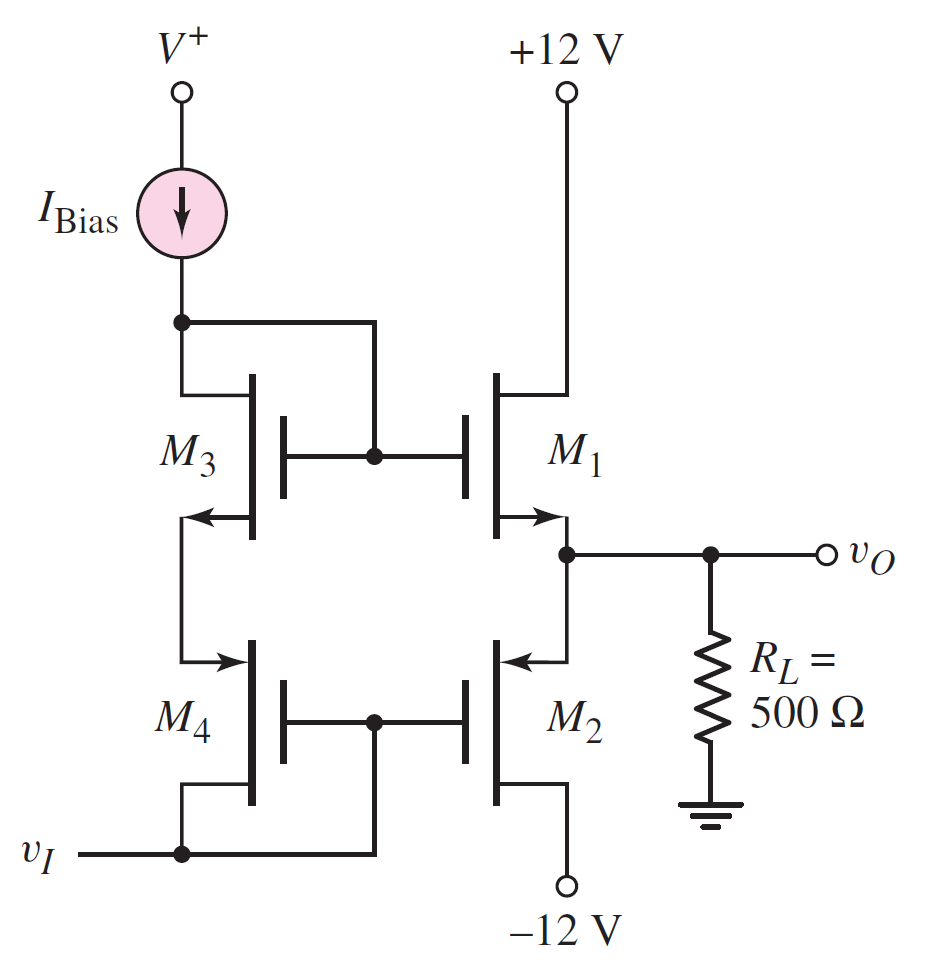
\includegraphics[width=0.5\textwidth]{8.29}
	\caption{Problem 8.29}
\end{figure}

\end{document}